\documentclass[]{interact}
\usepackage{amsmath,amssymb,amsfonts}
\usepackage{booktabs}
\usepackage{graphicx}
\usepackage{multirow}
\usepackage{url}
\usepackage[hidelinks]{hyperref}
\usepackage[authoryear]{natbib}
\bibpunct{(}{)}{,}{a}{}{,}
\renewcommand\bibfont{\fontsize{10}{12}\selectfont}

\begin{document}

\articletype{Research Article}

\title{When resolution consistency fails: an information-matched audit for disaster remote sensing}

\author{
\name{AKSHAY SHARMA\textsuperscript{a*} and LALJI PRASAD\textsuperscript{a}}
\affil{\textsuperscript{a}Department of Computer Science and Engineering, SAGE University, Indore, Madhya Pradesh 452020, India}
\thanks{*Corresponding author. Email: akssha74@gmail.com}
}

\maketitle

\noindent\textbf{Running head:} Auditing resolution reliability
\par\medskip

\begin{abstract}
Reliability scores under spatial-resolution shift are often compared without
checking whether they receive the same information. We audit a multi-scale
Jensen--Shannon consistency score that ranks errors on an eight-fold degraded
image while retaining access to its unavailable finer original. Exact-hash-
clean AIDER and Hurricane Damage splits, three independently trained ResNet-18
seeds per corpus, and matched confidence, energy, Earth-observation nearest-
neighbour, virtual-logit matching and received-image consistency baselines are
used. Removing the finer reference reduces mean consistency error area under
the receiver operating characteristic curve (AUROC) from
0.964 to 0.623 on AIDER and from 0.989 to 0.590 on Hurricane Damage.
The reference-dependent minus received-image AUROC gaps are 0.341 and 0.399,
respectively; all six seed-level 10,000-replicate paired bootstrap intervals
exclude zero. No
deployable score dominates across corpora and seeds, and native-calibrated
thresholds do not preserve both coverage and low selective risk. We then
prospectively replicate the anchor-matched gap with MobileNetV3-Small and four
resampling operators: all 36 architecture/corpus/operator seed intervals remain
positive. A reveal/mask experiment holding the anchor, fine-scale set and score
fixed passes all 24 combinations (minimum aligned-minus-masked gap 0.359;
maximum empirical probability 0.0099), identifying image-specific
fine-reference correspondence as a driver. Separately, we
replace overlapping geospatial crops with guarded blocks and evaluate 1,441
same-building UAS/post-event-satellite pairs from four acquisitions at three
geographies and two hurricane events. The intersection-controlled UAS
classifier exceeds the majority baseline for every seed. Received-image
consistency has a positive pooled satellite AUROC lift over confidence, but the
effect reverses at both Hurricane Michael acquisitions; spatial-cluster
intervals include zero. The mean-based threshold-transfer criterion passes,
but its post-hoc all-seed robustness sensitivity fails. A prospective
third-event sensitivity adds 458 Hurricane Idalia UAS/crewed-aircraft pairs
with 37 overlap clusters; mean received-consistency AUROC lift is 0.325 and all
three cluster intervals are positive. The findings show a
large oracle--received protocol gap and demonstrate that acquisition pooling
can reverse operational conclusions, while exact duplicates and spatial
overlap require explicit controls. We develop an information-set and leakage
audit protocol for resolution-reliability studies.

\end{abstract}

\section{Introduction}

Spatial resolution varies across uncrewed-aerial-system and satellite disaster
products because altitude, optics, acquisition geometry, mosaicking and
delivery constraints vary. A classifier can consequently encounter a coarse
image while remaining confident in an incorrect prediction. Selective
prediction and out-of-distribution (OOD) scores are intended to identify such
unreliable cases, but their evaluation is meaningful only when competing scores
receive the same information.

Multi-view disagreement is a plausible reliability signal. Predictive-
distribution divergences can forecast performance under distribution shift
\citep{schirmer2023divergence}, and Jensen--Shannon (JS) consistency has an
established role in corruption-robust training \citep{hendrycks2020augmix}.
However, a synthetic resolution ladder creates a specific failure mode. When
an error made on an eight-fold degraded image is scored by disagreement with
the retained undegraded original, the score receives a finer reference that a
system receiving only the coarse image does not possess. Comparing it with
confidence or feature distance from the coarse image conflates score quality
with information access.

Evaluation data can introduce a second form of optimism. Exact images can occur
across nominal splits, and fixed crops from nearby geospatial objects can share
source pixels even when object identifiers differ. Duplicate contamination is
known to bias image benchmarks \citep{barz2020cifair}, while spatial dependence
can substantially inflate remote-sensing accuracy estimates
\citep{karasiak2022spatial,kattenborn2022spatial}. These issues are especially
important for reliability studies because they change both classifier errors
and the apparent ability to rank those errors.

This article presents a pre-specified, failure-finding audit of reliability
under resolution shift. It makes four contributions:

\begin{enumerate}
\item It defines an information-set audit that contrasts
reference-dependent and received-image consistency for the same coarse-image
errors.
\item It compares maximum-softmax confidence, maximum logit, energy, Earth-
observation (EO) deep nearest neighbours, virtual-logit matching (ViM), and
received-image consistency under identical source-only information.
\item It replaces contaminated evaluations with encoded-byte duplicate
exclusion and guarded spatial blocks whose retained 512-pixel crops have zero
cross-split intersections.
\item It extends measured-ground-sampling-distance (GSD) evaluation to paired
UAS and post-event satellite buildings from four held-out acquisitions at
three geographies and two disaster events, with independent model seeds and
paired spatial-cluster uncertainty.
\end{enumerate}

The intended outcome is deployment guidance and an executable audit protocol,
not a claim that JS disagreement or any existing OOD score is a new primitive.
Negative and superseded results are retained as part of the evidence.

\section{Related work}

\subsection{Disagreement and reliability}

Predictive disagreement is widely used as a proxy for epistemic uncertainty.
\citet{schirmer2023divergence} show that full-distribution divergences, including
JS divergence, can be more informative than top-class agreement for performance
forecasting under shift. AugMix instead uses JS consistency as a training
objective across augmentations \citep{hendrycks2020augmix}. These precedents
mean that neither JS divergence nor transformation consistency is itself the
novelty of this study. The present question is whether a divergence-based score
has been evaluated with information unavailable at deployment.

Our verified literature set does not establish that this exact unavailable-
fine-reference comparison is prevalent in published EO practice. The failure
mode was exposed in a prior internal evaluation and is studied here as a
concrete counterexample and audit case, not as an estimate of field-wide
prevalence.

\subsection{OOD detection in Earth observation}

Remote-sensing OOD work considers unseen classes, sensors and geographical
domains. The remote-sensing Dirichlet prior network (DPN-RS) uses in-domain and
auxiliary OOD examples to learn distributional uncertainty
\citep{gawlikowski2022dpnrs}. Post-hoc alternatives
avoid additional OOD training. Deep nearest neighbours use distance to
normalised source features \citep{sun2022knn}; ViM combines a principal-space
feature residual with classifier logits \citep{wang2022vim}. A ten-method EO
benchmark found ViM and nearest neighbours among the strongest methods without
retraining \citep{li2024tenood}. We therefore include both, but distinguish
prediction-error detection from conventional binary in-/out-of-distribution
classification.

Target-assisted EO detectors answer a different information-budget question.
TARDIS uses known and wild-domain samples to construct an auxiliary shift
detector~\citep{ekim2025tardis}; allowing the evaluation pool as its wild set
would be transductive relative to our source-only scores. EarthShift supplies
real-world EO shift tasks, including spatial-resolution variation, rather than
a directly interchangeable per-image error score~\citep{doerksen2026earthshift}.
We therefore treat these as adjacent protocols and compare the strongest
source-only post-hoc methods under a common received-image budget.

\subsection{Leakage and spatial validation}

Near-duplicate removal changes measured performance on established image
benchmarks \citep{barz2020cifair}. Geospatial collections can contain even more
severe split duplication \citep{geospatialdedup2023}. Separately, nearby
remote-sensing observations are spatially dependent. Buffered or spatial
leave-one-out validation is needed when the intended inference concerns new
areas \citep{karasiak2022spatial}, and random hold-outs can overstate
convolutional-network performance \citep{kattenborn2022spatial}. Our audit
checks both encoded-image identity and source-pixel intersection between fixed
crops; these are complementary failure modes.

\section{Audit method}

\subsection{Information sets}

Let \(f\) be a classifier and
\(\boldsymbol{p}_{s}(\mathbf{x})\) its predictive distribution after
downsampling an original image by factor \(s\) and resizing it to the network
input. The evaluated coarse prediction is
\(\hat{y}_{8}=\arg\max_c p_{8,c}(\mathbf{x})\).

The reference-dependent consistency score is
\begin{equation}
D_{\mathrm{ref}}(\mathbf{x}) =
\frac{1}{3}\sum_{s\in\{2,4,8\}}
\operatorname{JS}\!\left(
\boldsymbol{p}_{1}(\mathbf{x}),
\boldsymbol{p}_{s}(\mathbf{x})
\right).
\end{equation}
It uses the retained \(s=1\) image while ranking errors made at \(s=8\).
Accordingly, we label it a privileged diagnostic.

For the deployable counterpart, let \(\mathbf{z}\) be the image actually
received at effective scale 8. Only further degradations of \(\mathbf{z}\) are
available:
\begin{equation}
D_{\mathrm{recv}}(\mathbf{z}) =
\frac{1}{3}\sum_{r\in\{2,4,8\}}
\operatorname{JS}\!\left(
\boldsymbol{p}_{1}(\mathbf{z}),
\boldsymbol{p}_{r}(\mathbf{z})
\right),
\end{equation}
which corresponds to effective original scales \(8,16,32,64\). Both scores
rank the same errors of \(\boldsymbol{p}_{1}(\mathbf{z})\). Their paired
error-detection AUROC difference,
\begin{equation}
\Delta_{\mathrm{oracle}} =
\operatorname{AUROC}(D_{\mathrm{ref}})
-\operatorname{AUROC}(D_{\mathrm{recv}}),
\end{equation}
is the descriptive oracle--received protocol gap rather than a method
improvement. It combines finer-reference access with a change in the absolute
degradation regime. A post-hoc mechanism sensitivity therefore anchors both
scores on the received \(s=8\) prediction, uses three comparisons in each
score, and contrasts finer views \(\{1,2,4\}\) with coarser views
\(\{16,32,64\}\). This sensitivity controls the anchor and comparison count but
still changes degradation direction; it is not interpreted causally.

\subsection{Matched deployable scores}

Every deployable score receives \(\mathbf{z}\), source training data and source
validation data only. We evaluate one minus maximum softmax probability,
negative maximum logit, energy, deep nearest-neighbour distance, ViM
\citep{wang2022vim}, and \(D_{\mathrm{recv}}\). The nearest-neighbour bank uses
normalised penultimate source features \citep{sun2022knn}; \(k\) is selected
from \(\{1,5,10,20,50\}\) by source-validation error AUROC. Let \(W\) and
\(\mathbf{b}\) denote the final linear classifier's weight matrix and bias
vector, and let \(W^{+}\) denote the Moore--Penrose pseudoinverse. ViM
constructs the classifier origin \(-W^{+}\mathbf{b}\), estimates a principal
source-feature subspace, and appends the scaled residual norm as a virtual OOD
logit. Its principal dimension is selected from
\(\{64,128,256,384\}\) using source validation only.
Both selections use labelled source-validation images degraded to the target
synthetic factor \(s=8\). This deliberately favourable, shift-specific
supervised tuning is reported separately from untuned confidence, max-logit and
energy scores.

\subsection{Leakage controls}

For AIDER and Hurricane Damage, we compute SHA-256 over encoded image bytes.
Every member of a cross-split hash group is excluded; conflicting-label groups
are reported explicitly. All other assignments remain fixed.

For CRASAR-U-DROIDs, 512-by-512 crops are centred on labelled buildings.
Source-image coordinates are partitioned into 2048-by-2048 blocks assigned
deterministically to training, validation or internal test sets. A crop is
retained only when its centroid lies at least 256 pixels inside every block
boundary. We then exhaustively test axis-aligned crop rectangles and require
zero intersections between different splits.

\subsection{Paired measured-GSD audit}

The measured-GSD evaluation pairs identical building identifiers with matching
eligible labels in UAS and post-event satellite products. Reliability is
computed separately from each received crop; no UAS view is supplied when
scoring its satellite pair. Thresholds at target coverages \(0.5\), \(0.7\)
and \(0.9\) are calibrated on guarded source validation and transferred
unchanged. We report realised coverage, absolute coverage error, selective
risk and false-critical rate.

All GSD values are read from the fixed CRASAR \texttt{statistics.csv}. The
exact dataset revision and metadata SHA-256 are recorded in the public
data-source ledger and released metadata manifest.

Uncertainty is estimated with 10,000 paired spatial-cluster bootstrap
replicates. Sites are top-level clusters and 2048-by-2048 UAS source blocks are
resampled within site, retaining every paired building in a sampled block.
A post-hoc dependence sensitivity additionally groups pairs into connected
components whenever either their UAS or satellite 512-pixel crop rectangles
overlap, and reports site-specific intervals. This stronger clustering is not
used to redefine the preregistered criteria.

\section{Experimental setup}

\subsection{Datasets}

AIDER version 1.0 (CC BY 4.0) supplies five disaster-scene classes and the
primary synthetic resolution audit~\citep{aiderdata}. Its corrected
train/validation/test counts are 4,499/961/969. Satellite Images of Hurricane
Damage (CC BY 4.0) supplies an independent binary corpus through the
fixed Hugging Face revision recorded in the public data-source ledger; corrected counts are
6,997/997/2,000~\citep{hurricanedata}. CRASAR-U-DROIDs (CC BY 4.0) provides
source coordinates, building-damage labels, measured GSD metadata, and aligned
UAS/satellite products at the fixed released revision~\citep{crasar2024data}.

The AIDER frozen split is corrected only by excluding every member of the two
conflicting-label exact-duplicate groups discovered by the pre-specified hash
audit. The Hurricane split uses the fixed seed-0 70/10/20 index assignment and
the same all-members exclusion rule for cross-split hashes.

Intersection-controlled CRASAR classifier training uses guarded crops from Lancaster Canyon
Gate (Hurricane Harvey) and Summerlin San Carlos (Hurricane Ian). The held-out
paired evaluation uses Harlem Heights and McGregor College Parkway South 1
(Hurricane Ian), plus the 13 and 14 October Mexico Beach products (Hurricane
Michael). A prospective third-event sensitivity pairs Steinhatchee River UAS
and post-event crewed-aircraft products from Hurricane Idalia. Evaluation
geographies do not contribute images, labels or outcomes to training or model
selection.

\subsection{Training}

The primary classifier is the ImageNet-1K-initialised
\texttt{microsoft/resnet-18} checkpoint at the revision recorded in the
environment manifest. We train independent seeds
101, 202 and 303 with AdamW (learning rate \(3\times10^{-4}\), weight decay
\(10^{-4}\)), batch size 64, and class-weighted cross-entropy. For class \(c\),
the loss weight is \(N/(C n_c)\), where \(N\) is the training-set size, \(C\)
the number of classes, and \(n_c\) the class count. The checkpoint with the
highest source-validation macro-F1 is retained. AIDER uses six epochs,
Hurricane Damage five, and intersection-controlled CRASAR 12.

Training first resizes to 256 pixels, then applies a random 224-pixel resized
crop with scale range 0.75--1.0 and a horizontal flip with probability 0.5.
Evaluation uses resize-to-256 and a 224-pixel centre crop. Both use ImageNet
channel normalisation. Synthetic resolution degradation uses bicubic
downsampling and upsampling before these transforms. Runs use Python 3.10.20,
PyTorch 2.12.1, torchvision 0.27.1, timm 1.0.28, Transformers 5.12.1 and
Apple M4 Max Metal Performance Shaders.

\subsection{Architecture and operator replication}

After independent review, we prospectively froze a second-architecture and
degradation-operator replication before training or test evaluation. Three
ImageNet-initialised \texttt{timm} MobileNetV3-Small-100 models use the same
clean AIDER split, seeds, optimiser, batch size and six-epoch schedule.
Bicubic, bilinear, nearest-neighbour and box down/up sampling are fixed.

For each architecture, seed and operator, errors are defined at \(s=8\). The
anchor-matched fine-reference score compares \(s=8\) with
\(\{1,2,4\}\), while received-image consistency compares \(s=8\) with
\(\{16,32,64\}\). We report 2,000-replicate paired intervals. The original
torchvision MobileNet weight endpoint returned HTTP 503 before any training;
the pre-evaluation addendum records the switch to
\texttt{timm==1.0.28}.

\subsection{Metrics and fixed analysis}

Error detection is evaluated with AUROC, area under the precision--recall curve
(AUPRC), and false-positive rate at 95\% error recall (FPR95). Classification
metrics include accuracy, balanced accuracy and macro-F1. Threshold-transfer
metrics are coverage, absolute target-coverage error, selective risk and
false-critical rate.

Paired score differences use 10,000 within-seed bootstrap replicates. The
measured-GSD analysis additionally uses the paired spatial-cluster bootstrap
defined above. Seed-level values and sample standard deviations are reported;
model-seed variation is not substituted for building- or site-sampling
uncertainty.

\subsection{Pre-specified criteria}

Criterion A1 requires positive privileged-minus-received mean AUROC on both
synthetic corpora, a positive paired bootstrap interval for every seed, and six
positive seed differences. W11 requires pooled held-out UAS accuracy above the
pooled majority baseline for all seeds and mean balanced accuracy of at least
0.60. W12 requires positive mean received-consistency lift on satellite views,
positive seed-specific spatial-cluster intervals, and positive mean lift at
three or more of four sites. W13 requires the mean satellite absolute coverage
error to be no larger for received consistency than confidence and the mean
received-consistency selective risk to be no higher at target coverage 0.70.
Requiring both inequalities for every seed is reported only as a post-hoc
robustness sensitivity.

The third-event E1 criterion requires mean held-out Idalia UAS balanced
accuracy of at least 0.55. E2 requires complete metrics, selection counts,
physical footprints, raw arrays and overlap-cluster uncertainty for all three
seeds; no ranking-sign or accuracy-direction criterion is imposed.

M1 requires positive bicubic MobileNet anchor-matched gaps and intervals for
all seeds. M2 extends the sign requirement to all four operators, with at least
two positive intervals per operator. M3 requires positive ResNet means and at
least two positive intervals for every corpus/operator combination. M4 requires
aligned fine-reference AUROC to exceed the mean of 100 correspondence-masked
permutations with empirical probability at most 0.05 for all 24
ResNet corpus/seed/operator combinations.

\section{Results}

\subsection{Duplicate audits and corrected training}

The encoded-byte audit found two cross-split AIDER hash groups. Both had
conflicting labels; excluding every member removed four images and left 6,429.
The Hurricane Damage audit found three cross-split groups with matching labels;
the all-members rule removed six images and left 9,994. No encoded-byte hash
remained in more than one split (Table~\ref{tab:hash-audit}).

\begin{table}[t]
\centering
\caption{Encoded-byte cross-split duplicate audit. Every member of each listed group was excluded before retraining.}
\label{tab:hash-audit}
\begin{tabular}{lrrr}
\toprule
Dataset & Groups & Excluded & Retained \\
\midrule
AIDER & 2 & 4 & 6429 \\
Hurricane Damage & 3 & 6 & 9994 \\
\bottomrule
\end{tabular}
\end{table}


\subsection{Oracle--received protocol gap}

The reference-dependent diagnostic and received-image consistency ranked the
same errors at effective scale 8 but differed in access to finer views. On
AIDER, their mean AUROCs were \(0.964\pm0.013\) and \(0.623\pm0.113\),
respectively. The mean oracle--received AUROC gap was \(0.341\pm0.120\).
On Hurricane Damage, mean AUROC changed from \(0.989\pm0.003\) to
\(0.590\pm0.045\), a gap of \(0.399\pm0.043\).

All six seed-level differences were positive. Every 10,000-replicate paired
bootstrap interval excluded zero: AIDER intervals ranged from
\([0.183,0.249]\) to \([0.415,0.495]\), and Hurricane intervals ranged from
\([0.330,0.378]\) to \([0.413,0.465]\)
(Table~\ref{tab:inflation}). The pre-specified A1 criterion therefore passed.

\begin{table}[t]
\centering
\caption{Paired oracle--received gap in error AUROC. Brackets give 95\% paired bootstrap intervals from 10,000 replicates.}
\label{tab:inflation}
\begin{tabular}{lcc}
\toprule
Seed & AIDER & Hurricane Damage \\
\midrule
101 & 0.351 [0.312, 0.391] & 0.354 [0.330, 0.378] \\
202 & 0.216 [0.183, 0.249] & 0.439 [0.413, 0.465] \\
303 & 0.455 [0.415, 0.495] & 0.405 [0.380, 0.430] \\
\bottomrule
\end{tabular}
\end{table}


Because the two primary protocols also differ in anchor and absolute
degradation regime, we ran a post-hoc mechanism sensitivity that anchors both
scores on \(s=8\) and uses three comparisons. Replacing the unavailable finer
views \(\{1,2,4\}\) with further degradations \(\{16,32,64\}\) produced mean
AUROC gaps of \(0.336\pm0.122\) on AIDER and \(0.398\pm0.044\) on Hurricane
Damage; all six paired intervals remained positive
(Table~\ref{tab:anchor-matched}). This controls anchor and comparison count,
but not degradation direction, and is reported as sensitivity evidence rather
than a new confirmatory endpoint.

\begin{table}[t]
\centering
\caption{Post-hoc anchor-matched mechanism sensitivity. Both scores anchor on the received $s=8$ prediction and use three comparisons; the table reports fine-reference minus further-degradation error AUROC with 95\% paired bootstrap intervals.}
\label{tab:anchor-matched}
\begin{tabular}{lcc}
\toprule
Seed & AIDER & Hurricane Damage \\
\midrule
101 & 0.346 [0.304, 0.387] & 0.351 [0.327, 0.375] \\
202 & 0.209 [0.175, 0.243] & 0.439 [0.413, 0.465] \\
303 & 0.452 [0.411, 0.493] & 0.404 [0.379, 0.429] \\
\bottomrule
\end{tabular}
\end{table}


\subsection{Prospective architecture and operator replication}

The second-architecture replication retained the anchor-matched gap for all
three MobileNetV3-Small seeds and all four operators. Mean MobileNet AIDER gaps
ranged from \(0.215\pm0.014\) (nearest-neighbour) to
\(0.465\pm0.260\) (bicubic). ResNet AIDER means ranged from
\(0.247\pm0.005\) to \(0.336\pm0.122\), and ResNet Hurricane means from
\(0.331\pm0.069\) to \(0.398\pm0.045\)
(Table~\ref{tab:architecture-operator}).

All 36 seed-level intervals across the three architecture/corpus series and
four operators excluded zero. Consequently, pre-specified criteria M1, M2 and
M3 passed. The gap is therefore not conditional on ResNet-18 or bicubic
resampling, although all operators still compare finer and coarser degradation
directions.

\begin{table}[t]
\centering
\caption{Prospective architecture/operator replication of the anchor-matched fine-reference minus received-image error-AUROC gap. Values are mean $\pm$ sample SD over three independently trained seeds.}
\label{tab:architecture-operator}
\resizebox{\textwidth}{!}{%
\begin{tabular}{lccc}
\toprule
Operator & MobileNet AIDER & ResNet AIDER & ResNet Hurricane \\
\midrule
Bicubic & 0.465 $\pm$ 0.260 & 0.336 $\pm$ 0.122 & 0.398 $\pm$ 0.045 \\
Bilinear & 0.420 $\pm$ 0.277 & 0.329 $\pm$ 0.129 & 0.331 $\pm$ 0.069 \\
Nearest & 0.215 $\pm$ 0.014 & 0.251 $\pm$ 0.033 & 0.367 $\pm$ 0.059 \\
Box & 0.244 $\pm$ 0.065 & 0.247 $\pm$ 0.005 & 0.349 $\pm$ 0.079 \\
\bottomrule
\end{tabular}}
\end{table}


\begin{figure}[t]
\centering
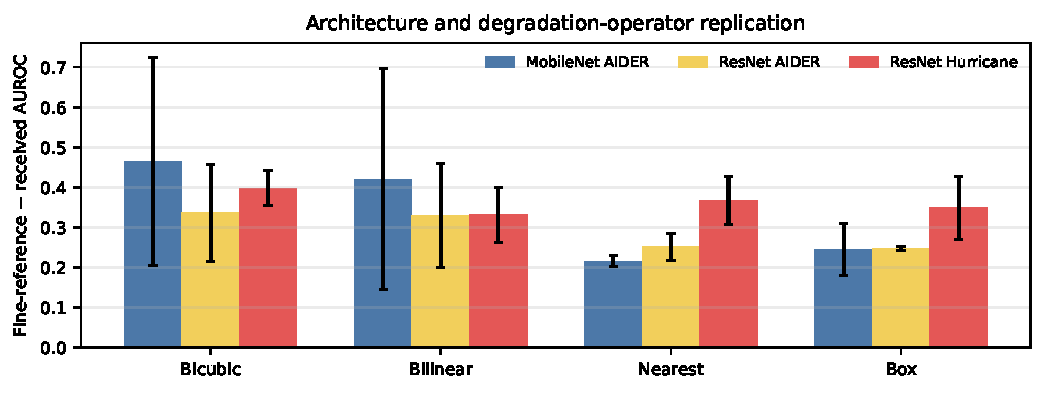
\includegraphics[width=\textwidth]{figures/architecture_operator_replication.pdf}
\caption{Prospective architecture and degradation-operator replication of the
anchor-matched fine-reference minus received-image error-AUROC gap. Bars show
mean across three independently trained seeds; error bars are sample SD.}
\label{fig:architecture-operator}
\end{figure}

\subsection{Fine-reference reveal/mask identification}

Aligned finer views exceeded correspondence-masked finer views in all 24
ResNet corpus/seed/operator combinations. The smallest aligned-minus-masked
mean AUROC gap was 0.359, and the largest empirical one-sided probability was
0.0099. M4 therefore passed.

Mean gaps across seeds ranged from \(0.365\pm0.005\) to
\(0.425\pm0.003\) on AIDER and from \(0.462\pm0.029\) to
\(0.490\pm0.004\) on Hurricane (Table~\ref{tab:reveal-mask}). Because masked
scores preserve the anchor, scale set, score functional, comparison count and
fine-prediction marginals, this result identifies image-specific fine/coarse
correspondence as a driver of the diagnostic advantage within the tested
protocol.

\begin{table}[t]
\centering
\caption{Pre-specified fine-reference reveal/mask experiment. Values are aligned-minus-masked-mean error AUROC across three ResNet seeds; the final column is the maximum empirical one-sided probability across both corpora and all seeds.}
\label{tab:reveal-mask}
\begin{tabular}{lccc}
\toprule
Operator & AIDER gap & Hurricane gap & Max. probability \\
\midrule
Bicubic & 0.371 $\pm$ 0.008 & 0.490 $\pm$ 0.004 & 0.0099 \\
Bilinear & 0.365 $\pm$ 0.005 & 0.469 $\pm$ 0.019 & 0.0099 \\
Nearest & 0.423 $\pm$ 0.006 & 0.482 $\pm$ 0.017 & 0.0099 \\
Box & 0.425 $\pm$ 0.003 & 0.462 $\pm$ 0.029 & 0.0099 \\
\bottomrule
\end{tabular}
\end{table}


\begin{figure}[t]
\centering
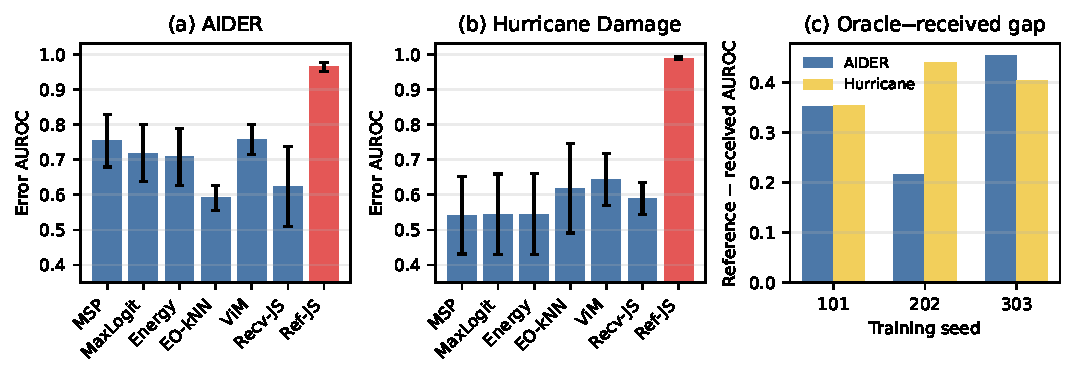
\includegraphics[width=\textwidth]{figures/information_audit.pdf}
\caption{Information-matched error detection. Bars in the first two panels are
mean AUROC across independent training seeds; error bars are sample SD. The red
bar is a non-deployable diagnostic with access to the retained finer reference.
The third panel shows its paired AUROC gap over received-image
consistency for every seed. MSP denotes maximum softmax probability; Recv-JS
and Ref-JS denote received-image and reference-dependent consistency.}
\label{fig:information-audit}
\end{figure}

\subsection{Matched deployable baselines}

Under matched received-image information, no consistency score dominated the
post-hoc baselines (Table~\ref{tab:matched-auroc}). ViM had the highest mean
AIDER AUROC (0.758), closely followed by confidence (0.754); received-image
consistency reached 0.623. On Hurricane Damage, ViM reached 0.643, EO-kNN
0.618, received-image consistency 0.590, and confidence 0.542. These rankings
varied by seed: received-image consistency exceeded confidence strongly for
Hurricane seed 101, was lower for seed 202, and was statistically
indistinguishable for seed 303. The evidence therefore supports the
oracle--received gap, not universal superiority of one deployable
score.

The preregistered paired ViM-minus-EO-kNN comparison was recomputed from
per-example arrays. All three AIDER intervals were positive
(\(0.132\) or greater at the lower bound). On Hurricane Damage, seed 101 was
positive, seed 202 was negative, and seed 303 included zero. ViM therefore did
not dominate EO-kNN across training runs.

\begin{table}[t]
\centering
\caption{Error-detection AUROC under matched received-image information. The final row is a non-deployable diagnostic with access to the retained finer reference. Values are mean $\pm$ sample SD across three independently trained seeds.}
\label{tab:matched-auroc}
\begin{tabular}{lcc}
\toprule
Score & AIDER & Hurricane Damage \\
\midrule
Confidence & 0.754 $\pm$ 0.075 & 0.542 $\pm$ 0.110 \\
Max logit & 0.718 $\pm$ 0.081 & 0.545 $\pm$ 0.114 \\
Energy & 0.708 $\pm$ 0.081 & 0.545 $\pm$ 0.115 \\
EO-kNN & 0.591 $\pm$ 0.035 & 0.618 $\pm$ 0.127 \\
ViM & 0.758 $\pm$ 0.043 & 0.643 $\pm$ 0.074 \\
Received consistency & 0.623 $\pm$ 0.113 & 0.590 $\pm$ 0.045 \\
Reference-dependent diagnostic & 0.964 $\pm$ 0.013 & 0.989 $\pm$ 0.003 \\
\bottomrule
\end{tabular}
\end{table}


\subsection{Threshold transfer}

Native-validation thresholds did not preserve both target coverage and low
selective risk under severe shift. At target coverage 0.70 on AIDER, mean
realised coverage was 0.384 for confidence, 0.257 for ViM, and 0.228 for
received-image consistency. ViM selected a lower-risk subset
(mean selective risk 0.040) but missed the target by 0.443 on average.

On Hurricane Damage, confidence, EO-kNN and ViM mean coverages were 0.029,
0.003 and below 0.001. Received-image consistency instead accepted 0.974 on
average, but its mean selective risk was 0.467. Thus high transferred coverage
did not indicate safe auto-decision retention. Reporting coverage without risk
would reverse the operational interpretation.

\subsection{Intersection-controlled measured-GSD replication}

The guarded CRASAR split retained 1,628 crops from two training sites: 975 for
training, 267 for validation and 386 for internal testing. Exhaustive rectangle
comparison found zero cross-split 512-pixel intersections. Internal test
accuracy was \(0.794\pm0.007\), above the 0.635 majority baseline for every
seed; balanced accuracy was \(0.781\pm0.013\).

The held-out paired evaluation contained 1,441 buildings in 708 UAS spatial
blocks across four acquisitions at three geographies and two hurricane events
(Table~\ref{tab:measured-gsd}).
Same-eligible-label selection retained 531/978 common identifiers at Harlem,
269/366 at McGregor, 337/507 at Mexico Beach 13 October, and 304/634 at Mexico
Beach 14 October. These exclusions are reported because the resulting sample
conditions on cross-product label agreement.
Pooled UAS accuracy was \(0.747\pm0.014\), above the 0.533 pooled majority
baseline for every seed, and balanced accuracy was \(0.752\pm0.014\).
Criterion W11 therefore passed. Satellite accuracy fell to
\(0.486\pm0.081\), below the same majority baseline on average, confirming a
severe cross-platform shift without invalidating the UAS classifier.

The post-hoc joint-overlap sensitivity connected pairs whenever either their
UAS or satellite crops overlapped. It produced two effective clusters at
Harlem and one at each remaining site because the larger satellite footprints
overlap extensively. Pooled intervals continued to include zero, while
site-specific cluster intervals were degenerate and are not interpreted as
independent site inference.

\begin{table}[t]
\centering
\caption{Intersection-controlled CRASAR classifier and pooled held-out paired results. Values are mean $\pm$ sample SD across seeds.}
\label{tab:crasar-summary}
\begin{tabular}{lc}
\toprule
Endpoint & Value \\
\midrule
Guarded internal accuracy & 0.794 $\pm$ 0.007 \\
Guarded internal majority accuracy & 0.635 \\
UAS accuracy & 0.747 $\pm$ 0.014 \\
Satellite accuracy & 0.486 $\pm$ 0.081 \\
Satellite confidence AUROC & 0.465 $\pm$ 0.067 \\
Satellite received-consistency AUROC & 0.614 $\pm$ 0.079 \\
\bottomrule
\end{tabular}
\end{table}

\begin{tabular}{lccccc}
\toprule
Measured GSD & Accuracy & Error conf. & AUROC$_{1-c}$ & AUROC$_{RCG}$ & Lift \\
\midrule
UAS 3.84--4.67\,cm\,px$^{-1}$ & 0.661$\pm$0.040 & 0.782$\pm$0.031 & 0.582$\pm$0.078 & 0.818$\pm$0.030 & 0.236$\pm$0.051 \\
Satellite 30.52\,cm\,px$^{-1}$ & 0.400$\pm$0.170 & 0.800$\pm$0.094 & 0.483$\pm$0.109 & 0.747$\pm$0.126 & 0.264$\pm$0.121 \\
\bottomrule
\end{tabular}


\begin{figure}[t]
\centering
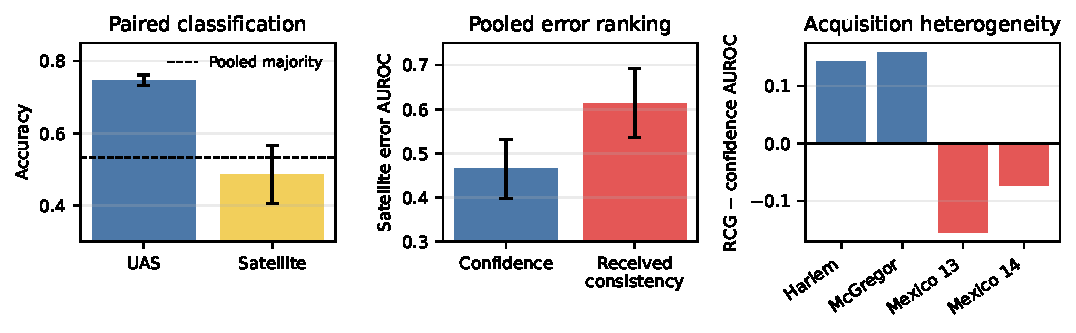
\includegraphics[width=\textwidth]{figures/measured_gsd_audit.pdf}
\caption{Intersection-controlled paired measured-GSD audit. Error bars in the first two
panels are sample SD across training seeds. The acquisition panel shows that the
pooled received-consistency advantage is confined to the two Hurricane Ian
sites and reverses at both held-out Hurricane Michael sites.}
\label{fig:measured-gsd}
\end{figure}

\subsection{Measured-GSD ranking and threshold transfer}

On pooled satellite views, received-image consistency reached error AUROC
\(0.614\pm0.079\), compared with \(0.465\pm0.067\) for confidence; all three
seed differences were positive and the mean difference was 0.149. This pooled
summary did not generalise by site. Mean differences were 0.143 at Harlem
Heights and 0.159 at McGregor, but \(-0.155\) and \(-0.073\) on the two
Mexico Beach sites. The paired spatial-cluster bootstrap intervals for the
pooled difference included zero for every seed. W12 therefore failed.

Measured threshold transfer was also heterogeneous. At target coverage 0.70,
received-image consistency achieved mean satellite coverage
\(0.701\pm0.138\), compared with \(0.499\pm0.068\) for confidence. Mean
selective risk was lower (0.456 versus 0.548), but seed 202 reversed this
ordering (0.549 versus 0.530), and spatial-cluster risk-difference intervals
included zero. The preregistered mean-based W13 therefore passed, while the
stricter post-hoc all-seed robustness sensitivity failed. The expanded
evaluation changes the conclusion from a positive two-site ranking result to
event-associated heterogeneity with no confirmatory ranking success and no
seed-uniform threshold-transfer robustness.

\subsection{Third-event Hurricane Idalia sensitivity}

The prospective third-event sensitivity retained 458/605 common Steinhatchee
River building identifiers with matching eligible UAS/crewed-aircraft labels.
Measured GSD was 12.70 and 15.02 cm\,px\(^{-1}\), so the 512-pixel crops span
approximately 65.0 and 76.9 m. Joint UAS/crewed overlap grouping yielded 37
clusters.

Mean held-out UAS balanced accuracy was 0.572, passing E1; absolute accuracy
remained below the 0.954 majority baseline because only 21 paired buildings
were damaged. E2 passed with complete raw outputs and cluster inference.
Received consistency exceeded confidence on crewed-aircraft errors by 0.312,
0.389 and 0.274 AUROC across seeds; all three 2,000-replicate cluster intervals
excluded zero and mean lift was 0.325 (Table~\ref{tab:idalia}). Accuracy
improved slightly for seed 101 and declined for seeds 202 and 303, consistent
with the pre-specified absence of an accuracy-direction criterion.

\begin{table}[t]
\centering
\caption{Prospective third-event Hurricane Idalia sensitivity on 458 same-building UAS/crewed-aircraft pairs. The final columns report received-consistency minus confidence error-AUROC and its joint-overlap-cluster bootstrap interval.}
\label{tab:idalia}
\begin{tabular}{lrrrr}
\toprule
Seed & UAS balanced acc. & Crewed balanced acc. & AUROC lift & 95\% CI \\
\midrule
101 & 0.593 & 0.621 & 0.312 & [0.261, 0.372] \\
202 & 0.527 & 0.578 & 0.389 & [0.210, 0.472] \\
303 & 0.596 & 0.570 & 0.274 & [0.142, 0.344] \\
\bottomrule
\end{tabular}
\end{table}


\section{Discussion}

The audit distinguishes a useful diagnostic question from a deployable
reliability claim. A reference-dependent score asks whether the prediction on a
coarse synthetic view disagrees with a finer image that the benchmark retains.
This can diagnose resolution sensitivity when both views genuinely exist. It
does not establish that a system receiving only the coarse image can reproduce
the same ranking or threshold-transfer behaviour.

Information matching changes the interpretation of baseline comparisons.
Confidence, energy, nearest-neighbour distance, virtual-logit matching, and
received-image consistency can all be computed from the received image plus
source data. Their relative performance therefore concerns the score rather
than hidden input access. A reference-dependent score is retained as an
explicit upper-information diagnostic, not presented as an operational
competitor.

The prospective replication strengthens the scope of this conclusion. Positive
anchor-matched gaps occur for ResNet-18 and MobileNetV3-Small under bicubic,
bilinear, nearest-neighbour and box resampling, with all 36 seed-level
intervals excluding zero. The mechanism is therefore robust to the tested
architecture and operator choices. It remains a directional
fine-versus-coarse comparison, not a causal estimate of information access.

The reveal/mask experiment addresses the narrower identification question.
When scale set, anchor, score and marginal fine predictions are fixed, breaking
only image correspondence reduces error AUROC in all 24 combinations.
Corresponding fine-reference information therefore drives the aligned
diagnostic within this intervention. This does not identify the entire
oracle--received gap, because deployment still substitutes coarser views rather
than permuted finer views.

The data audits have a related purpose. Exact duplicate checks target literal
reuse across splits, whereas guarded spatial blocks target shared pixels and
local spatial dependence between fixed crops. Neither control alone establishes
geographical generalisation. The held-out site and event design therefore
complements, rather than replaces, the lower-level leakage checks.

The multi-event result illustrates why pooling is insufficient. Received-image
consistency had a positive pooled satellite AUROC difference because the two
Hurricane Ian acquisitions favoured it, while both Hurricane Michael
acquisitions favoured confidence. Cluster intervals consequently included zero despite three
positive pooled seed differences. Likewise, mean threshold-transfer coverage
and risk favoured consistency, so preregistered W13 passed, but one seed
reversed the risk ordering and the post-hoc all-seed sensitivity failed.
Consequently, W12 does not support general ranking and W13 does not establish
seed-uniform robustness; the measured-GSD evidence supports event-associated
heterogeneity and audit practice rather than a winning gate.

The held-out Hurricane Idalia UAS/crewed comparison adds a third event, a
different aerial platform and substantially closer physical footprints than the
UAS/satellite pairs. Received consistency ranks crewed-aircraft errors above
confidence for all seeds with positive cluster intervals. This broadens the
real-world result, but the extreme undamaged majority and one Idalia geography
still preclude event-general operational claims.

\section{Limitations and threats to validity}

The synthetic ladder is a controlled image transformation, not a physical
sensor model. It isolates information access but does not recreate atmospheric,
optical or processing effects associated with a changed GSD. The paired
CRASAR comparison adds measured GSD but changes platform, sensor, view geometry,
processing and physical footprint together; it therefore supports a
cross-platform resolution-shift conclusion rather than a causal effect of GSD
alone.

The primary reference-dependent and received-image scores also differ in
absolute scale regime. Their AUROC difference is therefore a descriptive
oracle--received protocol gap, not an identified causal effect of reference
access alone. The anchor-matched sensitivity controls the anchor and comparison
count but still contrasts finer with coarser degradation directions.

The audit evaluates disaster scene and binary building-damage classifiers with
one backbone family. Three independent seeds quantify training variation but do
not establish architecture universality. The held-out measured-GSD sites cover
two hurricane events, not every hazard or geographical region. The two Mexico
Beach acquisitions share geography and the effective event-level sample size is
two; event-associated sign differences are descriptive rather than
event-general inference.

Paired buildings are restricted to identifiers with the same eligible label in
both products. This avoids label disagreement as an explanation for prediction
changes but conditions the sample on cross-product agreement; the resulting
class proportions are not population prevalence estimates. The protocol files,
local execution logs and hashes record that criteria were frozen before their
corresponding evaluations, but they were not deposited in an external
preregistration registry before execution. Independent external timestamp
verification is therefore unavailable.

ViM and nearest neighbours are strong source-only post-hoc baselines in EO
benchmarks, but methods trained with auxiliary OOD data answer a different
information-budget question. DPN-RS is consequently discussed rather than
mixed into the matched source-only ranking. Finally, exact hashes do not detect
all near-duplicates; the public release retains encoded hashes and feature
outputs so a future perceptual audit can extend the analysis.

\section{Conclusion}

Reliability comparisons under resolution shift require an explicit account of
what each score can observe. This study separates a reference-dependent
resolution diagnostic from scores that can be computed when only the received
image is available, then combines that information audit with exact-duplicate,
spatial-intersection and measured-GSD checks. The anchor-matched gap replicates
across ResNet-18, MobileNetV3-Small, four resampling operators and all 36
seed-level intervals; a fixed reveal/mask intervention identifies
image-specific fine-reference correspondence as a driver in all 24 tested
combinations. A third measured-GSD event supplies an additional
positive cluster-level ranking sensitivity. The resulting protocol is
designed to prevent an unavailable finer view or shared source pixels from
being mistaken for a stronger uncertainty method. Its practical recommendation
is simple: declare the inference-time information set, match it across
baselines, audit image identity and crop geometry, and retain failed
threshold-transfer results before making an operational reliability claim.


\section*{Acknowledgements}
During preparation of this work, the authors used the Cursor artificial-intelligence assistant with GPT-5.6 Sol for software-development assistance, reference checking, result verification, and language refinement. The authors reviewed the source and revised versions, checked all quantitative claims against the registered execution artefacts, and take full responsibility for the final manuscript. No artificial-intelligence tool is listed as an author, and no artificial-intelligence-generated image is included.

\section*{Funding}
No specific funding was received for this work.

\section*{Disclosure statement}
No competing interest was reported by the authors.

\section*{Data availability statement}
AIDER version 1.0 is available from Zenodo under CC BY 4.0 at \url{https://doi.org/10.5281/zenodo.3888300}~\citep{aiderdata}. Satellite Images of Hurricane Damage is available from IEEE DataPort and its documented Hugging Face mirror under CC BY 4.0 at \url{https://doi.org/10.21227/sdad-1e56}~\citep{hurricanedata}; this study fixes mirror revision \texttt{4bb60de01b2d9e323d364d76d8b08c2eaeef1a64}. CRASAR-U-DROIDs version 1 is available from DesignSafe-CI and Hugging Face under CC BY 4.0 at \url{https://doi.org/10.17603/ds2-fqy5-n314}~\citep{crasar2024data}; this study fixes revision \texttt{47cf4ab3a94d42978975f7d23338a996125ac0e9}. No third-party imagery is redistributed. Version 2.0.0 of the complete code and evidence package is available at \url{https://github.com/akssha74/rcg-tt} and archived under the version-independent DOI \url{https://doi.org/10.5281/zenodo.21510152}~\citep{auditsoftware}. The archive contains exact split files, portable per-example scores, source manifests, checkpoints, execution logs, claim and citation ledgers, and generated tables and figures. Code is MIT-licensed and generated research artefacts are CC BY 4.0.

\appendix
\section{Reproducibility and audit details}

The supplementary release records the encoded-byte hashes used for duplicate
audits, every excluded item, guarded-block coordinates, all retained crop
rectangles, and the exhaustive cross-split intersection result. Seed-level
checkpoints and raw score arrays are retained so that AUROC, AUPRC, FPR95,
threshold-transfer, and bootstrap calculations can be independently
recomputed.

Compressed per-example arrays contain labels, predictions and all synthetic
audit scores for every corpus/seed. The paired measured-GSD arrays additionally
contain UAS and satellite predictions, confidence, received consistency, site,
event, UAS block, satellite block and joint overlap-cluster identifiers.
Portable indexes omit local filesystem paths. The reproduction command verifies
their hashes, recomputes headline metrics and the preregistered W13
adjudication, regenerates publication artefacts and clean-builds the paper.

Failed and superseded branches remain part of the release. In particular, the
initial unpaired measured-GSD criterion, the overlapping-crop analysis, the
reference-dependent operational interpretation, and the failed
received-image-only W8/W9 experiment are not deleted when corrected evidence is
generated.

The first implementation applied an all-seed W13 rule although the frozen
criterion was mean-based. The corrected adjudication records W13 as passed and
the all-seed requirement as a failed post-hoc robustness sensitivity. Other
independent-review sensitivities, including anchor-matched finer-view scoring
and joint UAS/satellite overlap clustering, are explicitly labelled post hoc.

The structured information-set scoping audit is released as
\texttt{information\_set\_literature\_audit.json}. It records six search
queries, 12 included primary works, task/protocol classifications, and the
test-time information available to each method. The audit found no exact
published unavailable-fine-reference deployment comparison in this bounded
set; it is not presented as an exhaustive prevalence estimate.


\bibliographystyle{tfcad}
\bibliography{references}
\end{document}
